\documentclass[tikz,border=4pt]{standalone}
\usepackage{amsmath,amssymb}
\usetikzlibrary{arrows.meta,positioning,calc}
\begin{document}
    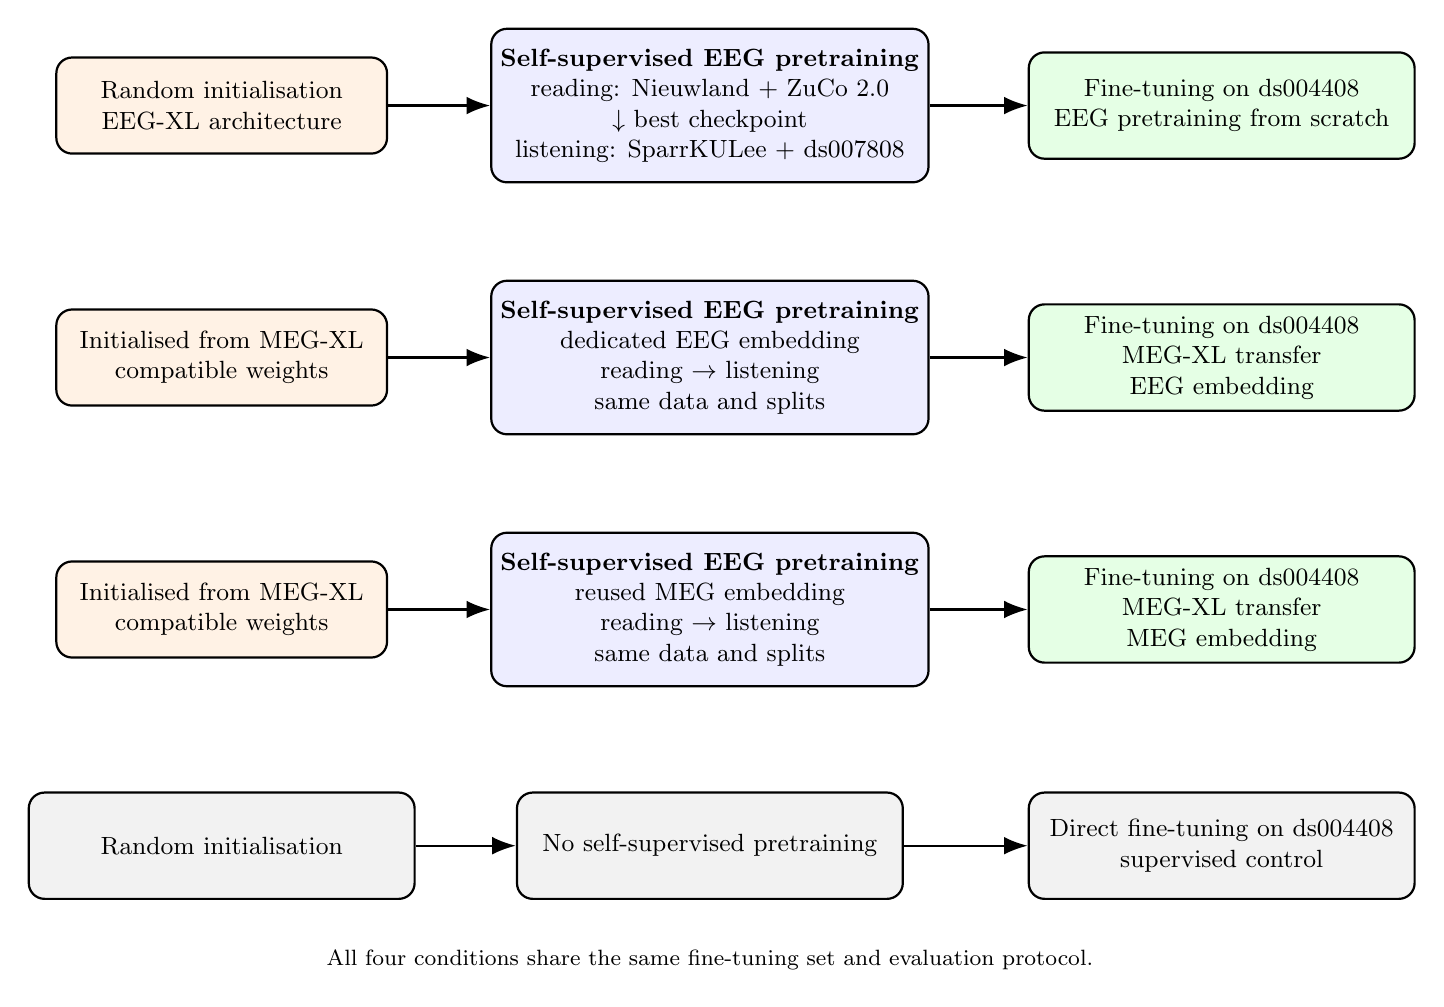
\begin{tikzpicture}[
        font=\small,
        arrow/.style={-{Latex[length=3mm]}, thick},
        init/.style={draw, rounded corners=2mm, minimum width=4.2cm,
                    minimum height=1.22cm, align=center, thick, fill=orange!10},
        conjunto/.style={draw, rounded corners=2mm, minimum width=5.4cm,
                          minimum height=1.95cm, align=center, thick, fill=blue!7},
        final/.style={draw, rounded corners=2mm, minimum width=4.9cm,
                     minimum height=1.35cm, align=center, thick, fill=green!10},
        control/.style={draw, rounded corners=2mm, minimum width=4.9cm,
                       minimum height=1.35cm, align=center, thick, fill=gray!10},
        note/.style={font=\footnotesize, align=center}
    ]
        \node[init] (scratchinit) at (0,5.4) {Random initialisation\\EEG-XL architecture};
        \node[conjunto] (scratchcurr) at (6.2,5.4) {\textbf{Self-supervised EEG pretraining}\\
              reading: Nieuwland + ZuCo 2.0\\
              $\downarrow$ best checkpoint\\
              listening: SparrKULee + ds007808};
        \node[final] (scratchft) at (12.7,5.4) {Fine-tuning on ds004408\\EEG pretraining from scratch};

        \node[init] (megeeginit) at (0,2.2) {Initialised from MEG-XL\\compatible weights};
        \node[conjunto] (megeegcurr) at (6.2,2.2) {\textbf{Self-supervised EEG pretraining}\\
              dedicated EEG embedding\\
              reading $\rightarrow$ listening\\
              same data and splits};
        \node[final] (megeegft) at (12.7,2.2) {Fine-tuning on ds004408\\MEG-XL transfer\\EEG embedding};

        \node[init] (megmeginit) at (0,-1.0) {Initialised from MEG-XL\\compatible weights};
        \node[conjunto] (megmegcurr) at (6.2,-1.0) {\textbf{Self-supervised EEG pretraining}\\
              reused MEG embedding\\
              reading $\rightarrow$ listening\\
              same data and splits};
        \node[final] (megmegft) at (12.7,-1.0) {Fine-tuning on ds004408\\MEG-XL transfer\\MEG embedding};

        \node[control] (directinit) at (0,-4.0) {Random initialisation};
        \node[control] (direct) at (6.2,-4.0) {No self-supervised pretraining};
        \node[control] (directft) at (12.7,-4.0) {Direct fine-tuning on ds004408\\supervised control};

        \draw[arrow] (scratchinit) -- (scratchcurr);
        \draw[arrow] (scratchcurr) -- (scratchft);
        \draw[arrow] (megeeginit) -- (megeegcurr);
        \draw[arrow] (megeegcurr) -- (megeegft);
        \draw[arrow] (megmeginit) -- (megmegcurr);
        \draw[arrow] (megmegcurr) -- (megmegft);
        \draw[arrow] (directinit) -- (direct);
        \draw[arrow] (direct) -- (directft);

        \node[note] at (6.2,-5.45) {All four conditions share the same fine-tuning set and evaluation protocol.};
    \end{tikzpicture}
\end{document}
